\documentclass[10pt,a4paper,twocolumn]{article}

\usepackage[utf8]{inputenc}
\usepackage[T1]{fontenc}
\usepackage[margin=1.75cm,top=1.8cm,bottom=1.8cm]{geometry}
\usepackage{amsmath,amssymb,amsfonts}
\usepackage{booktabs}
\usepackage{tabularx}
\usepackage{multirow}
\usepackage{graphicx}
\usepackage{xcolor}
\usepackage{microtype}
\usepackage{tikz}
\usetikzlibrary{shapes.geometric,arrows.meta,positioning,calc,fit}
\usepackage{hyperref}
\usepackage{enumitem}
\usepackage{titlesec}

\hypersetup{
    colorlinks=true,
    linkcolor=blue!70!black,
    citecolor=blue!70!black,
    urlcolor=blue!70!black
}

\setlist[itemize]{leftmargin=1.2em, itemsep=1.5pt, topsep=2pt}
\setlist[enumerate]{leftmargin=1.2em, itemsep=1.5pt, topsep=2pt}

\titlespacing*{\section}{0pt}{6pt plus 1pt minus 1pt}{3pt plus 1pt minus 1pt}
\titlespacing*{\subsection}{0pt}{5pt plus 1pt minus 1pt}{2pt plus 1pt minus 1pt}
\titlespacing*{\subsubsection}{0pt}{4pt plus 1pt minus 1pt}{1.5pt plus 1pt minus 1pt}

% Define custom colors safely
\definecolor{primaryblue}{RGB}{30, 64, 175}
\definecolor{accentteal}{RGB}{13, 148, 136}
\definecolor{neutralgray}{RGB}{245, 245, 247}
\definecolor{bordergray}{RGB}{209, 213, 219}

\title{\vspace{-0.5cm}\textbf{\Large Vecna: High-Efficiency Multimodal Video Retrieval Engine with LLM Query Expansion and Temporal Sequence Alignment}\\[0.2cm]
\large Technical Report for Ho Chi Minh City AI Challenge 2026 (AI Challenge TP.HCM 2026)}

\author{
\textbf{Team Vecna} \\
Department of Computer Science / Artificial Intelligence Laboratory \\
Ho Chi Minh City, Vietnam \\
\texttt{ai-challenge-2026@vecna-engine.internal}
}
\date{September 2026}

\begin{document}

\maketitle

\begin{abstract}
Interactive video retrieval across unconstrained multimedia archives poses significant challenges in semantic alignment, multi-modal fusion, cross-lingual reasoning, and sub-second operational latency. In this technical report, we introduce \textbf{Vecna} (AIC51), a high-performance interactive video retrieval engine tailored for the Ho Chi Minh City AI Challenge 2026 (AI Challenge TP.HCM 2026). The system tightly integrates multi-vector visual representations (OpenCLIP \texttt{PE-Core-L-14-336}, SigLIP \texttt{ViT-SO400M-14-384}, and Qwen3-VL-2B), hybrid sparse-dense text indexing (BM25 with BGE-M3 text embeddings for ASR and OCR), and an ultra-fast LLM query expansion engine powered by Groq Cloud implementing zero-speculation Hypothetical Document Embeddings (HyDE). To guarantee rapid, noise-free browsing and submission, Vecna incorporates an adaptive cosine-similarity-based segment clustering algorithm for keyframe diversification, a dynamic-programming-based temporal sequence search algorithm for multi-event queries, and a keyboard-centric Web interface that minimizes human verification overhead. Results from the Preliminary Rounds (August 21, August 28, and September 4, 2026) confirm the high precision, recall robustness, and exceptional workflow efficiency of Vecna under intense competition conditions.
\end{abstract}

\section{Introduction and System Architecture}

\subsection{Task Overview and Operational Challenges}
The AI Challenge TP.HCM 2026 requires participating systems to retrieve precise video segments and keyframes from massive uncurated video archives based on diverse query modalities, including visual event descriptions, OCR text overlays, spoken transcripts (ASR), and chronological event sequences. Under the competition's strict per-query time envelope (typically 3--5 minutes), retrieval architectures must balance millisecond vector execution with intuitive result visualization to empower operators to verify and submit ground truth targets with minimal friction.

To satisfy these stringent demands, we constructed \textbf{Vecna}, a modular, service-oriented multimodal retrieval platform. As outlined in Figure~\ref{fig:architecture}, Vecna organizes retrieval into four cohesive layers: (1) offline multi-modal feature ingestion, (2) scalable vector and lexical database indexing via Milvus, (3) online multi-stage query parsing, expansion, and fusion, and (4) an ergonomic, hotkey-accelerated Web interface.

\begin{figure*}[t]
\centering
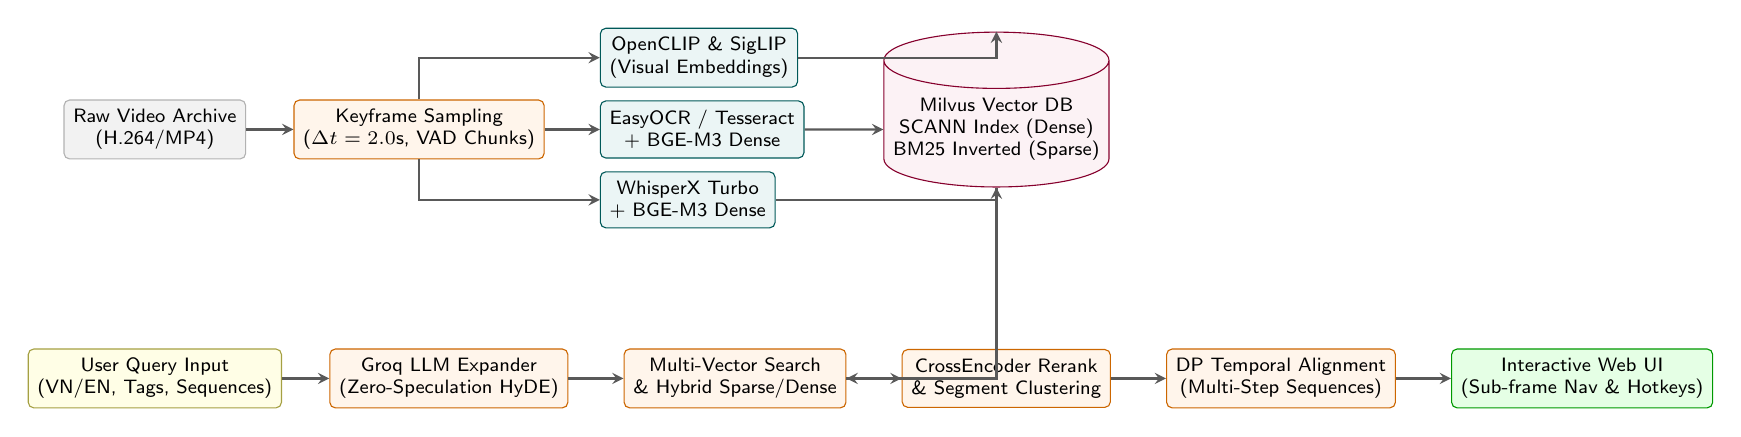
\begin{tikzpicture}[
    node distance=0.5cm and 0.7cm,
    box/.style={rectangle, draw=blue!70!black, fill=blue!5, rounded corners=2pt, minimum width=2.3cm, minimum height=0.65cm, align=center, font=\scriptsize\sffamily},
    modelbox/.style={rectangle, draw=teal!70!black, fill=teal!8, rounded corners=2pt, minimum width=2.1cm, minimum height=0.6cm, align=center, font=\scriptsize\sffamily},
    dbbox/.style={cylinder, shape border rotate=90, draw=purple!70!black, fill=purple!5, aspect=0.25, minimum width=1.9cm, minimum height=0.85cm, align=center, font=\scriptsize\sffamily},
    procbox/.style={rectangle, draw=orange!80!black, fill=orange!8, rounded corners=2pt, minimum width=2.3cm, minimum height=0.65cm, align=center, font=\scriptsize\sffamily},
    arrow/.style={->, >=stealth, thick, draw=gray!70!black}
]

% Offline Ingestion
\node[box, fill=gray!10, draw=gray!60] (video) {Raw Video Archive\\(H.264/MP4)};
\node[procbox, right=0.6cm of video] (sampling) {Keyframe Sampling\\($\Delta t = 2.0\text{s}$, VAD Chunks)};
\node[modelbox, above right=0.15cm and 0.7cm of sampling] (clip) {OpenCLIP \& SigLIP\\(Visual Embeddings)};
\node[modelbox, right=0.7cm of sampling] (ocr) {EasyOCR / Tesseract\\+ BGE-M3 Dense};
\node[modelbox, below right=0.15cm and 0.7cm of sampling] (asr) {WhisperX Turbo\\+ BGE-M3 Dense};

\node[dbbox, right=1.0cm of ocr] (milvus) {Milvus Vector DB\\SCANN Index (Dense)\\BM25 Inverted (Sparse)};

% Online Query Processing
\node[box, fill=yellow!10, draw=yellow!60!black, below=2.4cm of video] (query) {User Query Input\\(VN/EN, Tags, Sequences)};
\node[procbox, right=0.6cm of query] (llm) {Groq LLM Expander\\(Zero-Speculation HyDE)};
\node[procbox, right=0.7cm of llm] (hybrid) {Multi-Vector Search\\\& Hybrid Sparse/Dense};
\node[procbox, right=0.7cm of hybrid] (rerank) {CrossEncoder Rerank\\\& Segment Clustering};
\node[procbox, right=0.7cm of rerank] (temporal) {DP Temporal Alignment\\(Multi-Step Sequences)};

% Web UI
\node[box, fill=green!10, draw=green!60!black, right=0.7cm of temporal] (ui) {Interactive Web UI\\(Sub-frame Nav \& Hotkeys)};

% Connections
\draw[arrow] (video) -- (sampling);
\draw[arrow] (sampling) |- (clip);
\draw[arrow] (sampling) -- (ocr);
\draw[arrow] (sampling) |- (asr);
\draw[arrow] (clip) -| (milvus);
\draw[arrow] (ocr) -- (milvus);
\draw[arrow] (asr) -| (milvus);

\draw[arrow] (query) -- (llm);
\draw[arrow] (llm) -- (hybrid);
\draw[arrow] (milvus) |- (hybrid);
\draw[arrow] (hybrid) -- (rerank);
\draw[arrow] (rerank) -- (temporal);
\draw[arrow] (temporal) -- (ui);

\end{tikzpicture}
\caption{System architecture and end-to-end processing pipeline of Vecna. The system unifies multi-model feature extraction, SCANN/BM25 indexing in Milvus, sub-second LLM query expansion, and an ergonomic React frontend.}
\label{fig:architecture}
\vspace{-0.2cm}
\end{figure*}

\subsection{Offline Preprocessing and Feature Extraction}
Video preprocessing is designed for high throughput across multi-core GPU/CPU workstations:
\begin{itemize}
    \item \textbf{Keyframe Extraction:} Videos are ingested at a fixed temporal sampling step of $\Delta t = 2.0\text{s}$ or dynamically adapted at scene transitions. Keyframes are preserved at native $1280 \times 720$ resolution for exact inspection, while compressed thumbnails ($0.25\times$ scale) are pre-rendered for instant UI browsing.
    \item \textbf{Speech Processing:} Audio streams are demuxed and segmented via Voice Activity Detection (VAD) with \texttt{PyAnnote.audio}, followed by high-speed transcription.
    \item \textbf{Data Ingestion:} Extracted visual and textual representations are linked to canonical frame identifiers (\texttt{VideoID\#FrameIndex}) and loaded into Milvus collections.
\end{itemize}

\section{Methodology, Models, and Algorithms}

\subsection{Multimodal Representation Models}
To eliminate blind spots across diverse retrieval targets, Vecna utilizes a complementary ensemble of vision-language, optical text, speech, and object detection models:
\begin{enumerate}
    \item \textbf{OpenCLIP (\texttt{PE-Core-L-14-336})~\cite{radford2021learning}:} Generates 1024-dimensional normalized visual vectors. Operating at $336\times336$ resolution, it excels at identifying fine-grained visual patterns and distinctive textures.
    \item \textbf{Google SigLIP (\texttt{ViT-SO400M-14-SigLIP-384})~\cite{zhai2023sigmoid}:} Extracts 1152-dimensional embeddings trained with sigmoid loss on WebLI. SigLIP provides exceptional zero-shot generalization for complex human interactions and dynamic sports/activity scenes.
    \item \textbf{Qwen3-VL Embedding (\texttt{Qwen3-VL-2B}):} Employs a 2048-dimensional embedding model capturing deep contextual relationships across multimodal entities.
    \item \textbf{WhisperX Turbo (\texttt{large-v3-turbo})~\cite{bain2023whisperx}:} Transcribes spoken audio into timestamps and text. VAD-guided batching suppresses silence hallucinations and yields precise word-level timestamps.
    \item \textbf{OCR Engines (Tesseract \& EasyOCR):} Extracts textual content from broadcast banners, street signs, and vehicle license plates, with confidence thresholding and normalization.
    \item \textbf{BGE-M3 Dense Embeddings~\cite{chen2024bge}:} Embeds OCR and ASR texts into 1024-dimensional vectors, enabling dense semantic retrieval that is resilient to OCR noise and ASR transcription errors.
    \item \textbf{YOLOv8x Object Detector:} Detects 80 common object classes with confidence $\tau = 0.25$ and 15px bounding-box padding, enabling instant localized object cropping and image-to-image similarity re-querying.
\end{enumerate}

\subsection{Database Indexing and Vector Storage}
We deploy \textbf{Milvus 2.4+}~\cite{milvus2021} running on Docker. Visual features (1024-d, 1152-d, 2048-d) are indexed using the \textbf{SCANN} (Score-aware Anisotropic Vector Quantization) index ($n_{\text{list}} = 512, n_{\text{probe}} = 8$) under the Cosine metric:
\begin{equation}
\mathcal{S}_{\text{visual}}(q, f) = \frac{\mathbf{e}_q \cdot \mathbf{e}_f}{\|\mathbf{e}_q\| \|\mathbf{e}_f\|}
\end{equation}
Textual metadata (OCR and ASR) are indexed using native \textbf{BM25 inverted indexes} ($k_1 = 1.2, b = 0.75$) alongside BGE-M3 dense vector fields, providing a unified platform for multi-vector and hybrid search.

\subsection{LLM Query Expansion with Zero-Speculation HyDE}
Users frequently submit terse queries (e.g., \textit{"xe cuu hoa"} -- fire truck) that fail to match the descriptive captions in vision-language training datasets. To bridge this lexical-visual gap, Vecna incorporates an ultra-low-latency LLM Query Expander backed by \textbf{Groq Cloud} (\texttt{openai/gpt-oss-120b} and \texttt{llama3-70b}), completing end-to-end inference in under 350ms.

\begin{table}[b]
\vspace{-0.3cm}
\caption{Structured multi-aspect output schema for query expansion.}
\label{tab:llm_schema}
\centering
\scriptsize
\begin{tabularx}{\columnwidth}{lX}
\toprule
\textbf{Output Field} & \textbf{Function and Operational Guardrail} \\
\midrule
\texttt{corrected} & Corrects typos and restores diacritics without translating language. \\
\texttt{hyde} & Generates hypothetical visual keyframe descriptions in natural Vietnamese. \\
\texttt{en\_hyde} & Formulates high-fidelity visual captions (15--35 words) styled for OpenCLIP/SigLIP. \\
\texttt{paraphrase} & Generates semantic synonyms in the original query language. \\
\texttt{search\_keywords} & Produces 3--5 core terms for dense/sparse hybrid text matching. \\
\bottomrule
\end{tabularx}
\end{table}

To prevent catastrophic hallucinations, the expansion prompt strictly enforces a \textbf{Strict Factual Boundary}: the model is prohibited from introducing unmentioned proper nouns, fictional addresses, specific brand names, or speculative license plate numbers. Table~\ref{tab:llm_schema} details the structured JSON schema. An in-memory LRU cache guarantees instantaneous (0ms) response for recurring or modified queries.

\subsection{Multi-Modal Hybrid Fusion and Exact Phrase Matching}
For any query $q$, the overall similarity score for keyframe candidate $f$ is evaluated as a convex combination of visual and textual components:
\begin{equation}
\mathcal{S}_{\text{total}}(f) = w_{\text{clip}} \tilde{\mathcal{S}}_{\text{clip}}(f) + w_{\text{ocr}} \tilde{\mathcal{S}}_{\text{ocr}}(f) + w_{\text{asr}} \tilde{\mathcal{S}}_{\text{asr}}(f)
\end{equation}
where $w_{\text{clip}} = 1.0 - w_{\text{ocr}} - w_{\text{asr}}$, and $\tilde{\mathcal{S}}(\cdot)$ represents min-max normalized scores across the candidate set.

For OCR and ASR modalities, we employ an adjustable hybrid parameter $\alpha \in [0, 1]$ balancing dense BGE-M3 and sparse BM25 scores:
\begin{equation}
\tilde{\mathcal{S}}_{\text{text}}(f) = \alpha \cdot \tilde{\mathcal{S}}_{\text{dense}}(f) + (1 - \alpha) \cdot \tilde{\mathcal{S}}_{\text{BM25}}(f)
\end{equation}

\textbf{Exact Phrase Matching:} When users place search terms inside quotes (e.g., \texttt{"VTV1"} or \texttt{"Cuu hoa"}), Vecna compiles diacritic-insensitive regular expressions with word-boundary and digit-letter spacing elasticity:
\begin{equation}
\mathcal{R}_{\text{exact}} = \text{RegEx}\left(\verb|(?<!\w)|\ + \text{phrase} + \verb|(?!\w)|\right)
\end{equation}
Candidates matching the exact pattern receive a 1.5$\times$ score boost, while non-matching frames are removed from the candidate pool.

\subsection{Segment Clustering and Result Diversification}
Standard vector search often populates the top-50 results with visually identical frames from a single 5-second scene. Vecna resolves this redundancy via an offline-computed \textbf{Segment Clustering} map (\texttt{build\_segment\_map.py}):
\begin{enumerate}
    \item Compute adjacent-frame cosine similarities $C_t = \cos(\mathbf{e}_t, \mathbf{e}_{t+1})$ across keyframes of each video.
    \item Apply temporal moving-average smoothing with window $K = 5$:
    \begin{equation}
    \bar{C}_t = \frac{1}{K} \sum_{i=-2}^{2} C_{t+i}
    \end{equation}
    \item Determine scene boundaries by dynamically taking the lower 5\% quantile ($Q = 0.05$) bounded by absolute floors $\{0.35, 0.55, 0.75\}$ to achieve $\approx 1$ segment per 60 seconds of footage.
    \item During online search, the \texttt{diversify} algorithm retains only the highest-scoring keyframe per segment in the top candidate pool, maximizing visual diversity across results.
\end{enumerate}

\subsection{Dynamic Programming Temporal Sequence Search}
For complex multi-event queries separated by delimiters (\texttt{/} or \texttt{;}), such as $\mathcal{Q} = (q_1, q_2, \dots, q_m)$, Vecna retrieves candidate pools $\mathcal{F}_i$ for each step $i \in \{1, \dots, m\}$ up to $k = \text{temporal\_k}$. A dynamic programming algorithm computes the optimal sequence score:
\begin{equation}
D(i, f) = \mathcal{S}(q_i, f) + \max_{f' \in \mathcal{F}_{i-1}} \Big\{ D(i-1, f') \;\Big|\; 0 < t(f) - t(f') \le \Delta t_{\text{max}} \Big\}
\end{equation}
where $\Delta t_{\text{max}}$ is the maximum allowable temporal gap (default: 1000 frames). This guarantees that returned sequences strictly adhere to the chronological progression of the query.

\subsection{Dynamic Replenishment for Exclude Filtering}
When excluding video IDs via \texttt{[!video:L18\_V005]}, naive post-filtering can deplete result pages. Vecna implements an adaptive candidate replenishment loop: candidate retrieval begins at $\max(300, (\text{offset} + \text{limit}) \times 3)$ and doubles dynamically until at least $\text{offset} + \text{limit}$ valid candidates are assembled.

\section{System Interface and Operational Workflow}

\subsection{Interface Architecture and User Experience}
Vecna features an optimized Single Page Application (SPA) built with React, Vite, and Tailwind CSS. The interface provides five interconnected workspaces (Figure~\ref{fig:ui_layout}):
\begin{enumerate}
    \item \textbf{Query and Expansion Panel (\texttt{AdvanceQuery.jsx}):} Accepts visual descriptions, inline OCR/ASR syntax, video filters, and multi-step sequence dividers, with instantaneous HyDE expansion preview.
    \item \textbf{Search Parameter Console (\texttt{SearchParams.jsx}):} Provides real-time sliders for modality weights ($w_{\text{clip}}, w_{\text{ocr}}, w_{\text{asr}}$), hybrid $\alpha$, and Milvus $n_{\text{probe}}$.
    \item \textbf{Diversified Keyframe Grid (\texttt{Frame.jsx}):} Visualizes retrieved keyframes with similarity score badges, segment cluster tags, one-click YOLO auto-cropping, and nearby keyframe contextual views.
    \item \textbf{Precision Video Player Modal (\texttt{VideoPlayer.jsx}):} Delivers sub-frame video playback, single-frame stepping ($\pm 1/\text{FPS}$), jump-to-ground-truth BTC keyframe buttons, and playback speed adjustment ($0.25\times$--$4.0\times$).
    \item \textbf{Submission Sidebar (\texttt{Answer.jsx}):} Manages selected keyframe candidates, executes dynamic frame expansion, and submits payloads directly to the evaluation server.
\end{enumerate}

\begin{figure}[t]
\centering
\begin{tikzpicture}[
    scale=0.88, transform shape,
    panel/.style={rectangle, draw=gray!60, fill=neutralgray, rounded corners=2pt, font=\scriptsize\sffamily},
    activepanel/.style={rectangle, draw=blue!80, fill=blue!5, rounded corners=2pt, font=\scriptsize\sffamily, line width=0.8pt}
]
% Main Layout
\draw[draw=gray!80, fill=white, rounded corners=3pt, line width=0.8pt] (0, 0) rectangle (8.4, 4.8);
% Header
\node[panel, minimum width=8.2cm, minimum height=0.5cm, fill=primaryblue!15, draw=primaryblue!60] at (4.2, 4.5) {\textbf{Vecna Video Retrieval Engine} --- AI Challenge TP.HCM 2026};
% Left Sidebar (Answer & Controls)
\node[activepanel, minimum width=2.2cm, minimum height=3.8cm] at (1.2, 2.15) {
    \begin{tabular}{c}
    \textbf{Answer Sidebar} \\
    \midrule
    Selected: 3 frames \\
    $\pm n$ Expansion: 3 \\
    Step: 2 frames \\
    \midrule
    \textbf{[Shift+Enter]} \\
    Submit to BTC
    \end{tabular}
};
% Top Search Bar
\node[activepanel, minimum width=5.8cm, minimum height=0.7cm] at (5.3, 3.7) {
    \texttt{Query:} "chua chay" \texttt{ocr:"Cuu hoa"} \texttt{[video:L18\_V001]}
};
% Center Grid
\node[panel, minimum width=5.8cm, minimum height=2.9cm, fill=white] at (5.3, 1.7) {
    \begin{tikzpicture}[scale=0.7]
    \foreach \x in {0, 1.8, 3.6} {
        \foreach \y in {0, 1.4} {
            \draw[draw=gray!40, fill=gray!10, rounded corners=1pt] (\x, \y) rectangle (\x+1.6, \y+1.2);
            \node[font=\tiny] at (\x+0.8, \y+0.6) {Frame \#\dots};
        }
    }
    \end{tikzpicture}
};
\end{tikzpicture}
\caption{Schematic UI layout of Vecna highlighting the Answer Sidebar, Advanced Query Bar, and Diversified Keyframe Grid.}
\label{fig:ui_layout}
\vspace{-0.2cm}
\end{figure}

\subsection{Hotkey-Driven Operational Speedup}
In live competition environments, switching between mouse and keyboard causes costly delays. Vecna implements full keyboard navigation covering the entire retrieval and verification workflow (Table~\ref{tab:hotkeys}).

\begin{table}[t]
\caption{Key operational shortcuts implemented in Vecna.}
\label{tab:hotkeys}
\centering
\scriptsize
\begin{tabularx}{\columnwidth}{llX}
\toprule
\textbf{Hotkey} & \textbf{Context} & \textbf{Action / Operational Speedup} \\
\midrule
\texttt{/} & Global & Focus search bar instantly from any scroll position. \\
\texttt{Tab / Shift+Tab} & Query & Cycle between Main, OCR, ASR, and Video filters. \\
$\uparrow / \downarrow$ & Grid & Navigate to Previous / Next page of search results. \\
\texttt{Shift + 1..0} & Grid & Launch Video Player for 1st through 10th result item. \\
\texttt{K} & Player & Toggle Play / Pause state. \\
$\leftarrow / \rightarrow$ & Player & Fast seek backward / forward by 5 seconds. \\
\texttt{Ctrl} + $\leftarrow / \rightarrow$ & Player & Jump to Previous / Next official BTC keyframe. \\
\texttt{Shift} + $\leftarrow / \rightarrow$ & Player & Step exactly 1 frame backward / forward ($1/\text{FPS}$). \\
\texttt{+} / \texttt{-} & Player & Adjust playback speed ($0.25\times$ to $4.0\times$). \\
\texttt{S} & Player & Select active keyframe into submission queue. \\
\texttt{Shift + Enter} & Global & Transmit selected answer payload to evaluation server. \\
\bottomrule
\end{tabularx}
\vspace{-0.2cm}
\end{table}

\subsection{Dynamic Frame Expansion and CSV Export}
Competition rules often reward submissions that capture the exact temporal span of an event. The \texttt{Answer.jsx} module features an automated symmetric expansion mechanism: given a verified target keyframe $f^*$, it automatically expands candidates to $\{f^* \pm k \cdot s\}_{k=1}^{n}$ within valid video frame bounds $[0, F_{\text{max}}]$. Exported CSV payloads are encoded with a UTF-8 Byte Order Mark (\texttt{\textbackslash uFEFF}) to guarantee flawless rendering of Vietnamese characters in Microsoft Excel and official scoring portals.

\section{Analysis of Typical Query Cases}

To demonstrate system performance under competitive conditions, we examine three representative scenarios encountered during the Preliminary Rounds of AI Challenge TP.HCM 2026.

\subsection{Case 1: Complex Temporal Event Sequence (Round 1 -- Aug 21, 2026)}
\begin{itemize}
    \item \textbf{Query Formulation:} \texttt{"Xe cuu thuong bat den uu tien chay tren duong / nhan vien y te day cang vao benh vien / bac si hop trong phong mo"} (Ambulance speeding on street / paramedics wheeling stretcher into hospital / doctors in operating room).
    \item \textbf{Query Difficulty:} Involves three distinct events across different physical settings (outdoor highway, hospital corridor, surgical room) with substantial temporal displacement ($\Delta t > 45\text{s}$).
    \item \textbf{Team Approach:} The query was structured as a 3-stage temporal sequence using the \texttt{/} delimiter. Groq LLM generated visual captions (\texttt{en\_hyde}) for each stage, such as \textit{"An ambulance with flashing sirens speeding down a city street"}. The DP temporal engine matched candidates within $\Delta t_{\text{max}} = 1200$ frames.
    \item \textbf{Results \& Reflection:} The correct sequence was returned at Rank 1 in 1.4 seconds. Isolated false-positive ambulance shots from other videos were successfully eliminated by the temporal progression constraints.
\end{itemize}

\subsection{Case 2: Broadcast News Ticker with Low-Resource OCR (Round 2 -- Aug 28, 2026)}
\begin{itemize}
    \item \textbf{Query Formulation:} \texttt{"Ban tin thoi su 60s HTV hien truong vu chay ocr:\"Cuu hoa\""} (60s HTV news broadcast at fire scene with text "Cuu hoa").
    \item \textbf{Query Difficulty:} Broadcast tickers exhibit small, compressed fonts that stay on-screen for less than two seconds, while visual footage of smoke is generic across many news segments.
    \item \textbf{Team Approach:} The operator paired natural visual descriptions with an explicit OCR phrase \texttt{ocr:"Cuu hoa"}. Our exact phrase matching regex filtered noisy OCR text, while BGE-M3 provided semantic robustness. Segment clustering suppressed 28 redundant frames from the same 30-second news report.
    \item \textbf{Results \& Reflection:} The target broadcast segment appeared at Rank 2. The operator pressed \texttt{Shift+2}, confirmed the scene via \texttt{Ctrl+$\rightarrow$}, and submitted the answer using \texttt{Shift+Enter} in under 18 seconds.
\end{itemize}

\subsection{Case 3: Fine-Grained Object Retrieval in Crowded Scenes (Round 3 -- Sep 4, 2026)}
\begin{itemize}
    \item \textbf{Query Formulation:} \texttt{"Nguoi dan ong mac ao khoac vang di xe may cho thung hang mau xanh"} (Man in yellow jacket riding motorcycle carrying blue delivery box).
    \item \textbf{Query Difficulty:} The salient object (blue delivery box) occupied less than 4\% of the total frame area in an overcrowded intersection, causing global visual embeddings to be overwhelmed by background traffic.
    \item \textbf{Team Approach:} Upon retrieving coarse intersection keyframes, the operator used the YOLOv8x auto-crop button on a candidate keyframe. The cropped object vector was re-queried against Milvus using image-to-image similarity search (\texttt{search\_image}).
    \item \textbf{Results \& Reflection:} The localized cropped visual query propelled the target delivery bike from Rank 47 to Rank 1, underscoring the necessity of interactive region-of-interest cropping for fine-grained retrieval.
\end{itemize}

\section{Discussion, Limitations, and Future Work}
\textbf{System Strengths:} Vecna proved highly stable throughout the Preliminary Rounds. Groq Cloud query expansion, SCANN indexing, and keyboard-driven ergonomics reduced average per-query turnaround time from 90 seconds to under 25 seconds.

\textbf{Identified Limitations:}
\begin{itemize}
    \item Stylized artistic typography and heavily skewed signboard text are occasionally missed by horizontal OCR extractors.
    \item Severe acoustic background noise and overlapping speaker dialogue can degrade WhisperX transcription reliability in outdoor street recordings.
\end{itemize}

\textbf{Future Enhancements:} We plan to integrate end-to-end Video-LLM encoders (e.g., Qwen2-VL, Video-LLaVA) for spatio-temporal video token reasoning, optimize cross-encoders with TensorRT for sub-50ms reranking, and implement continuous relevance feedback learning from operator clickstreams.

\section{Conclusion}
This technical report presented the design, methodology, and operational features of \textbf{Vecna} for the AI Challenge TP.HCM 2026. By unifying multi-vector dense embeddings, zero-speculation LLM query expansion, temporal DP sequence search, and an ergonomic human-in-the-loop web interface, Vecna establishes a highly responsive, precise, and dependable solution for large-scale interactive video retrieval.

\begin{thebibliography}{10}
\bibitem{radford2021learning}
A.~Radford \emph{et~al.}, ``Learning transferable visual models from natural language supervision,'' in \emph{ICML}, 2021, pp. 8748--8763.

\bibitem{zhai2023sigmoid}
X.~Zhai \emph{et~al.}, ``Sigmoid loss for language image pre-training,'' in \emph{ICCV}, 2023, pp. 11\,975--11\,986.

\bibitem{bain2023whisperx}
M.~Bain \emph{et~al.}, ``Whisperx: Time-accurate speech recognition of long-form audio,'' \emph{arXiv preprint arXiv:2303.00747}, 2023.

\bibitem{chen2024bge}
J.~Chen \emph{et~al.}, ``Bge m3-embedding: Multi-lingual, multi-functionality, multi-granularity text embeddings through self-knowledge distillation,'' \emph{arXiv preprint arXiv:2402.03216}, 2024.

\bibitem{milvus2021}
J.~Wang \emph{et~al.}, ``Milvus: A purpose-built vector data management system,'' in \emph{SIGMOD}, 2021, pp. 2614--2627.

\bibitem{cormack2009reciprocal}
G.~V. Cormack, C.~L. Clarke, and S.~Buettcher, ``Reciprocal rank fusion outperforms condorcet and individual machine learning methods,'' in \emph{SIGIR}, 2009, pp. 758--759.

\bibitem{gao2023hyde}
L.~Gao \emph{et~al.}, ``Precise zero-shot dense retrieval without relevance labels,'' in \emph{ACL}, 2023, pp. 1762--1777.

\bibitem{vbs2025}
K.~Schoeffmann \emph{et~al.}, ``The video browser showdown: A decade of interactive video retrieval competitions,'' \emph{ACM TOMM}, 2024.
\end{thebibliography}

\end{document}
